\section{Results obtained}\label{sec:results}
\IEEEPARstart{T}{he} first result we managed to obtain is the index created by Lucene. For visualization of it, we used the tool called Luke that allows you to show the content.

\begin{figure}[H]
    \centering
    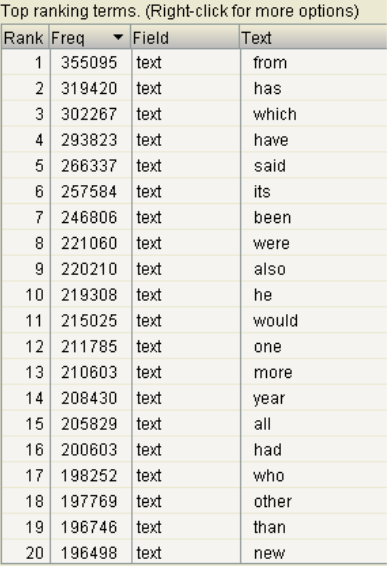
\includegraphics[width=0.6\columnwidth]{luke-1}
    \caption[Index]{Index shown with Luke}
    \label{fig:index}
\end{figure}

The following table illustrates the first 8 documents relating to the term '\textit{from}', term with rank 1 in the transposed index. The documents in the example are sorted by decreasing value of tf * idf.

\begin{figure}[H]
    \centering
    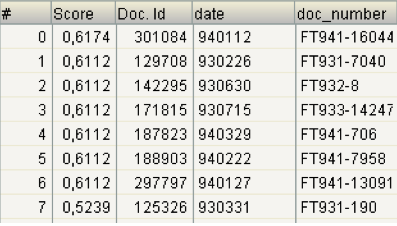
\includegraphics[width=0.6\columnwidth]{luke-2}
    \caption[Query]{Simplest query ever with Luke}
    \label{fig:query}
\end{figure}

The results of the basic Language Model are as follows:

\begin{table}[H]
    \centering
    \normalsize
    \begin{tabularx}{\columnwidth}{YYYY}
        \toprule
        \textbf{Topic Set} & \textbf{MAP} & \textbf{GMAP} & \textbf{RECALL}\\
        \midrule
        \textit{TREC-6} & 0.1612 & 0.0843 & 0.5382\\
        \midrule
        \textit{TREC-7} & 0.1734 & 0.0843 & 0.5444\\
        \midrule
        \textit{TREC-8} & 0.1899 & 0.0906 & 0.5484\\
        \midrule
        \textit{Robust} & 0.2021 & 0.1016 & 0.6052\\
        \bottomrule
    \end{tabularx}
    \caption{Results of basic LM}
    \label{tab:risultatiTestCollaudo}
\end{table}

We found minimal differences between the values ​​in the LM paper and the values ​​obtained from our implementation of the basic language model (Jelinek-Mercer).
We hypothesized the following reasons:
\begin{itemize}
\item Our indexing uses Lucene's standard stoplist. The paper does not specify whether the removal of the stopwords has been performed and with which stoplist;
\item we used Lucene's standard parser to get usable queries to get statistics related to the Jelinek-Mercer language model. This implementation may have changed but we have not studied in depth on GitHub (Lucene is open source and it is possible to perform a check), or in the paper they may have used their own implementation for parsing queries;
\item We don't know if a stemming was done in the base language model. We didn't do it.
\end{itemize}

As far as GLM is concerned, we were unable to reproduce the results due to the excessive time needed to extrapolate the k nearest neighbors from the used word2vec pretrained dataset (glove.6B.50d.txt). Although one of the smallest, it has a too high dimensionality for the time available.

\begin{figure}[H]
    \centering
    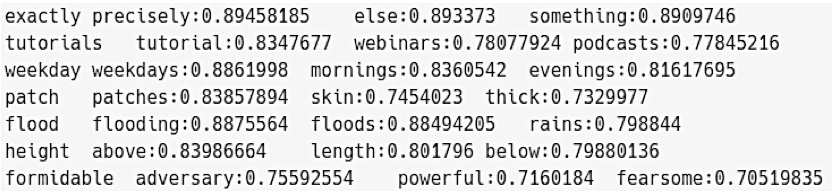
\includegraphics[width=\columnwidth]{knn}
    \caption[Knn]{Example of found k-nearest-neighbors}
    \label{fig:query}
\end{figure}

Leaving aside the aspect of computationally long times, the final formula for the calculation of probabilities has been reproduced in order to have a complete implementation at the code level.